\section{Marco teórico}
En 1949, \citeauthor{beauviour1949segundosexo} reconoció que existe una diferencia entre el sexo biológico\footnote{El sexo biológico es la distinción de los cuerpos entre un cuerpo de hombres o uno de mujer. El sexo se sigue entendiendo como binario (a excepción de Alemania que recientemente reconoció jurídicamente la existencia de cuerpos intersexuales) y es definido principalmente por los genitales externos. Sin embargo, el sexo está determinado por los cromosomas sexuales, la anatomía, las hormonas, el sistema reproductivo y otros \citep{lindsey2015genderroles}.} y la construcción social de cómo se debe vivir ese sexo. A partir de esto, planteó la crítica de que, para las mujeres, la biología es destino.\footnote{\cite{beauviour1949segundosexo} se enfoca en la construcción social de lo femenino pues argumenta que lo masculino fue construido como lo universal, que la mujer se define en oposición al hombre.} Es decir, que el hecho de nacer biológicamente mujer, implica un trato, una crianza y unas condiciones sociales que la define socialmente como mujer y la obligan a ejercer su feminidad. Posteriormente, \cite{butler2002gendertrouble} reformó el concepto sobre la de biología como destino y estableció que la cultura es destino para mujeres y hombres. La cultura opera para volverse destino de tres maneras. En primer lugar, la cultura crea normas que asocian el sexo biológico con el género como construcción social. En segundo lugar, ha generado un oposición entre lo masculino y lo femenino como atributos de hombres y mujeres, respectivamente. Por último, la cultura, al crear la asociación sexo-género y la oposición femenino-masculino, crea una concepción de coherencia de género a través de la que el género se convierte en un discurso preformativo del sexo \citep{butler2002gendertrouble}.

Lo anterior sugiere que hay acciones, comportamientos y actitudes asociadas de manera binaria a un género. Es a través de estas acciones que el género se vuelve un discurso preformativo. Las normas sociales que asocian las acciones, los comportamientos y las actitudes a un sexo-género para mantener la coherencia de género, se conocen como roles de género \citep{lindsey2015genderroles}. Cuando una acción se asocia a lo masculino, esa acción se entiende como una expresión de género masculina y cuando una acción se asocia a lo femenino se entiende como expresión de género femenina.

Para fines de este trabajo, los roles de género ($\mathbf{RG}$) son la función que va del espacio de acciones al espacio de géneros; donde el espacio de géneros ($\mathbf{G}$) como construcción social es binario. 
\begin{framed}
\noindent Sea $RG$ la función roles de género, $RG: A \rightarrow G$ tal que $G=\{f,m\}$
\end{framed}
Entonces, el conjunto de expresiones de género femeninas $(\mathbf{E_f})$ contiene todas las acciones que la función $RG$ mapea al género femenino y el conjunto de expresiones de género masculinas $(\mathbf{E_m})$ contiene todas las acciones que la función $RG$ mapea al género masculino. El conjunto de expresiones de género femeninas y el conjunto de expresiones de género masculinas, son disjuntos. Es decir, si una acción es considerada expresión de género (está en el dominio de RG), esa acción puede ser expresión femenina o expresión masculina, pero no puede ser femenina y masculina al tiempo. 

\begin{framed}
\noindent Sea $E_f$ el conjunto de expresiones de género femeninas y $E_m$ el conjunto de expresiones de género masculinas, $\forall k \in \{f, m\}, E_k=\{a_i\in A | RG(a_i)=k  \}$ tal que $E_f \cap  E_m=\varnothing$
\end{framed}

Por otra parte, la identidad de género ($\boldsymbol{I}$) es la concepción de sí mismo o, en términos de \cite{butler2002gendertrouble}, la designación psíquica del yo como un cuerpo con género (\textit{gendered body}). Bajo esta definición, la identidad de género no está limitada al conjunto de géneros binarios. De hecho, el conjunto de identidades de género puede llegar a tener tantos elementos como el número de personas que existan. En este trabajo, el conjunto de identidades de género contiene los géneros binarios y el género ``otro'' que agrupa los géneros no binarios. 

\begin{framed}
\noindent Sea $I$ el conjunto de identidades de género, $I=\{f,m,o\}$ y sea $\iota_j$ la identidad de la persona j, $\iota_j \in I$  
\end{framed}

Note que, siguiendo las definiciones de expresiones e identidades de género, las acciones son entendidas como expresiones de género de manera independiente a la identidad de la persona que toma dicha acción. 

A pesar de que ``no existe una identidad de género detrás de las expresiones de género'' \citep[p.~25]{butler2002gendertrouble}, existe una norma social ($\boldsymbol{\mathbb{P}}$) que ata la identidad de género con las expresiones y que prescribe los comportamientos socialmente adecuados \citep{akerlof2000economics}. Esa norma social exige que una persona que se identifique femenina tenga expresiones femeninas y una que se identifique masculina tenga expresiones masculinas. Es decir, $\boldsymbol{\mathbb{P}}$ es la correspondencia que va del espacio de identidades al espacio de expresiones de género. El dominio de  $\boldsymbol{\mathbb{P}}$ se limita a los género binarios, dado que al crear la asociación sexo-género de manera binaria, la norma social no se le asigna a las identidades no binarias un comportamiento adecuado. Por lo tanto, como las identidades no binarias no están en el dominio de $\mathbb{P}$, siempre que una persona de identidad otra, tome una acción que sea expresión de género, se entiende que está violando la norma social. 

\begin{framed}
\noindent Sea $\mathbb{P}$ la correspondencia norma social, $\mathbb{P}: I \twoheadrightarrow E$ tal que $\forall k \in \{f, m\}$, $\mathbb{P}(k)= E_k$ y $E=\{E_f,E_m\}$  
\end{framed}
La existencia de $\mathbf{\mathbb{P}}$ afecta la utilidad que deviene una persona, tanto cuando decide sus expresiones de género, como cuando interactúa con otra persona, dependiendo de si esa persona sigue o no la norma social. Por lo tanto, $\mathbf{\mathbb{P}}$ también afecta la disposición a interactuar con otros. 

Para ilustrar cómo las normas sociales de género pueden afectar la disposición a interactuar con otros, considere un juego de dos jugadores $N=\{1,2\}$ con información incompleta sobre la identidad de uno de los jugadores. Por simplicidad, solo el jugador 1 tiene identidad, $\iota_1 \in I$; por lo tanto, solo este jugador puede actuar acorde o contrario a $\mathbb{P}$. La naturaleza define que con probabilidad de 0.495 el jugador 1 se identifica femenino, con la misma probabilidad se identifica masculino y con probabilidad 0.01 se identifica con otra identidad.\footnote{\cite{meerwijk2017transgender} realizaron un estudio para calcular cuantas personas con identidad no binaria hay en los Estados Unidos. Los autores encuentran que las personas que no se identifican de manera binaria puede ser alrededor de 0.39\% de la población total. Los mismo autores mencionan que en otros lugares se ha calculado que ese porcentaje es cercano de 1.1\% y 0.8\%. Para este trabajo se toma 1\% por facilidad matemática y como aproximación al percentil más cercano de la cuota superior que se ha encontrado.} 
El jugador 1 conoce su identidad y debe decidir si toma una acción que sea una expresión de género femenina o una que sea masculina; el jugador 2 recibe esa señal, forma creencias sobre la identidad del jugador 1 y debe decir si interactúa o no con él. El conjunto de acciones del jugador 1 es $\mathbf{A_1}=\{E_f, E_m \}$; para fines del juego,  $E_f, E_m$ son singletons. El conjunto de acciones del jugador 2 es $\mathbf{A_2}=\{\text{Interactuar } (i), \text{No interactuar }(ni)\}$.

Al jugador 1, en ausencia de normas sociales, le genera una utilidad $\nu$ tener una expresión de género femenina y utilidad $0$ tener una expresión masculina. Sea $k \in~\{f,m\},$ la utilidad de cada expresión de género, en ausencia de normas sociales es: 
\begin{align*}
 \Pi_1(E_k)=   
\begin{cases}
    \nu & \text{si} \ k=f \\
    0 & \text{si} \ k=m
\end{cases}
\end{align*}
Al jugador 2 interactuar le genera una utilidad de $0$, mientras que no interactuar tiene un costo de $\eta>0$. Siguiendo el modelo prototipo de \cite{akerlof2000economics}, si el jugador 1 viola $\mathbb{P}$, su utilidad presenta una reducción en $\xi\geq0$.  Por ejemplo, si el jugador 1 se identifica masculino y decide pintarse la uñas (expresión de género femenina), en ausencia del normas sociales, su utilidad sería $\Pi_1(E_f)=\nu$.  Como consecuencia de que existe $\mathbb{P}$, su utilidad se vuelve  $\Pi_1(E_f|\iota_1=M; \mathbb{P})=\nu-\xi$, que es la utilidad que le genera pintarse la uñas, condicional a que está violando $\mathbb{P}$.

Además, cuando el jugador 1 viola $\mathbb{P}$, y los jugadores interactúan, el jugador 1 le genera una externalidad negativa de $\theta>0$ al jugador 2. Siguiendo el ejemplo anterior, si el jugador 2 interactúa con el jugador 1 de identidad masculina, que se pinta las uñas, la utilidad del jugador 2 es $\Pi_2(a_1=E_f, a_2=i|\iota_1=M; \mathbb{P})=-\theta$.

Dado que las acciones del jugador 1 pueden generar una externalidad sobre el jugador 2, este último puede decidir no interactuar con el jugador 1 para así restaurar parcialmente su utilidad en $\eta>0$ (el costo de no interactuar). Cuando el jugador 2 decide no interactuar con el jugador 1, la utilidad del jugador 1 se reduce en $\beta>0$. En el ejemplo anterior, si el jugador 2 decide no interactuar con el jugador 1, de identidad masculina, que se pinta las uñas,   los pagos son: $\Pi_1(a_1=E_f, a_2=ni|\iota_1=M; \mathbb{P})=\nu-\xi-\beta,\ \Pi _2(a_1=E_f, a_2=ni|\iota_1=M; \mathbb{P})=-\eta$. En la Figura \ref{fig:arbol} está representado el juego en forma extensiva. 

\begin{figure}[ht!]
	\caption{Representación extensiva}
	\label{fig:arbol}
	\centering
	\begin{tikzpicture}[-,auto,node distance=3cm,thick,
	main node/.style={fill=black, scale=0.1, draw,font=\sffamily\small\bfseries},
	sub node/.style={font=\sffamily\small\bfseries}, 
	primer node/.style={circle,draw, scale=0.5, font=\sffamily\small\bfseries}]
	
	\node[primer node](F){};
		\node[above] at (F){$\iota_1=F$};
		\node[below] at (F){$\{.495\}$};
	\node[main node](F1)[left = 2.5 cm of F]{1};
		\node[sub node](FNC1)[above left = 1.7 cm of F1]{};
			\node[below left] at (FNC1){$(\nu,0)$};
		\node[sub node](FC1)[below left = 1.7 cm of F1]{};
			\node[above left] at (FC1){$(\nu-\beta, -\eta)$};	
	\node[main node](F2)[right = 2.5 cm of F]{1};
		\node[sub node](FNC2)[above right = 1.7 cm of F2]{};
			\node[below right] at (FNC2) {$(-\xi,-\theta)$};
		\node[sub node](FC2)[below right = 1.7 cm of F2]{};
			\node[above right] at (FC2) {$(-\xi-\beta,-\eta)$};	

	\node[primer node](M)[below = 3 cm of F]{};
		\node[above] at (M){$\iota_1=M$};
		\node[below] at (M){$\{.495\}$};
	\node[main node](M1)[left = 2.5 cm of M]{1};
		\node[sub node](MNC1)[above left = 1.7 cm of M1]{};
			\node[below left] at (MNC1){$(\nu-\xi, -\theta)$};
		\node[sub node](MC1)[below left = 1.7 cm of M1]{};
			\node[above left] at (MC1){$(\nu-\xi- \beta,-\eta)$};
	\node[main node](M2)[right = 2.5 cm of M]{1};
		\node[sub node](MNC2)[above right = 1.7 cm of M2]{};
			\node[below right] at (MNC2){$(0,0)$};
		\node[sub node](MC2)[below right = 1.7 cm of M2]{};
			\node[above right] at (MC2) {$(-\beta,-\eta)$};
		
	\node[primer node](O)[below = 3 cm of M]{};
		\node[above]at (O){$\iota_1=O$};
		\node[below]at (O){$\{.01\}$};
	\node[main node](O1)[left = 2.5 cm of O]{1};
		\node[sub node](ONC1)[above left = 1.7 cm of O1]{};
			\node[below left] at (ONC1) {$(\nu-\xi,-\theta)$};
		\node[sub node](OC1)[below left = 1.7 cm of O1]{};
			\node[above left] at (OC1) {$(\nu-\xi-\beta,-\eta)$};
	\node[main node](O2)[right = 2.5 cm of O]{1};
		\node[sub node](ONC2)[above right = 1.7 cm of O2]{};
			\node[below right] at (ONC2){$(-\xi,-\theta)$};
		\node[sub node](OC2)[below right = 1.7 cm of O2]{};
			\node[above right] at (OC2) {$(-\xi- \beta, -\eta)$};
		
	\path[thick]
	(F)  edge node [above left]{$E_f$}(F1)
		 edge node [above right]{$E_m$}(F2)
	(F1) edge node [above right]{$i$}(FNC1)
		 edge node [below right]{$ni$}(FC1)
	(F2) edge node [above left]{$i$}(FNC2)
		 edge node [below left]{$ni$}(FC2)	 
	(M)  edge node [above left]{$E_f$}(M1)
		 edge node [above right]{$E_m$}(M2)
	(M1) edge node [above right]{$i$}(MNC1)
		 edge node [below right]{$ni$}(MC1)
	(M2) edge node [above left]{$i$}(MNC2)
	 	 edge node [below left]{$ni$}(MC2)			
	(O)  edge node [above left]{$E_f$}(O1)
		 edge node [above right]{$E_m$}(O2)
	(O1) edge node [above right]{$i$}(ONC1)
		 edge node [below right]{$ni$}(OC1)
	(O2) edge node [above left]{$i$}(ONC2)
		 edge node [below left]{$ni$}(OC2);
		 
	\draw[gray, dashed](F1)--(M1);
	\draw[gray, dashed](M1)--(O1);
	\draw[gray, dashed](F2)--(M2);
	\draw[gray, dashed](M2)--(O2);  	 	
	\end{tikzpicture}
	\begin{singlespace}
          \floatfoot{\footnotesize{\textit{Nota:} Esta figura representa un juego de información imperfecta en el que el jugador 1 puede ser de identidad $\{ F, M,O \}$. Ese jugador puede tomar una acción que es expresión de género femenina $(E_f)$ o masculina $(E_m)$. El jugador 2 al observar una expresión de género, forma creencias sobre la identidad del jugador 1 y decide si interactúa $(i)$ o no interactúa $(ni)$ con este. En ausencia de normas sociales, $\nu$ es la utilidad de tomar una expresión de femenina y la utilidad de tomar una expresión masculina es $0$. Si el jugador 1 rompe la norma social, percibe una desutilidad de $\xi$, y si interactúa con el jugador 2, le genera al jugador 2 una  externalidad de $\theta$. Si el jugador 2 decide no interactuar, percibe un costo de $\eta$ y le genera una externalidad al jugador 1 de $\beta$. }\par}
\end{singlespace}
\end{figure}

Al inicio del juego, el jugador 1 conoce su identidad y decide si tiene una expresión femenina o una masculina. El jugador 2 al observar la expresión de género del jugador 1, forma unas creencias sobre la identidad del jugador 1 y decide si interactúa o no. Los equilibrios bayesianos de Nash de este juego dependen de: (i) la utilidad relativa que le genera al jugador 1, dada su identidad, tener una expresión femenina frente a una expresión masculina (incorporando que el jugador 2 podría decidir no interactuar con él); y de (ii) la relación entre el costo de no interactuar y el costo esperado de observar que se viola la prescripción social. 

Existen seis posibles equilibrios bayesianos de Nash, cuatro agrupadores y dos separadores,\footnote{Un equilibrio es agrupador cuando independiente de la identidad, el jugador 1 toma la misma acción y un equilibrio es separador cuando la acción que toma el jugador 1 depende de su identidad.} que dependen de los parámetros poblacionales. Debido a que en los datos no se observan equilibrios agrupadores, esta sección expondrá únicamente los separadores.\footnote{El apéndice A expone los equilibrios agrupadores. El proceso de solución del modelo está disponible por solicitud.}

Existen equilibrios separadores, en estrategias puras, solo si las personas de identidad binaria cumplen la norma social. Es decir, el juego puede llegar a un equilibrio cuando el jugador 1 de identidad femenina (masculina) toma una expresión femenina (masculina). Bajo esa estrategia del jugador 1, el jugador 2 se enfrenta a dos posibilidades: (i) observa una expresión de género $E_k$ que toma el jugador 1 de una identidad binaria $k$ y el de identidad no binaria $(o)$, u (ii) observa una expresión de género $(E_{-k}$) que solo toma el jugador 1 de identidad binaria $-k$, donde $k \in \{f,m\}$. Para ambos casos, la mejor respuesta del jugador 2 es no interactuar solo si el costo de no interactuar es menor al costo esperado de que se viole la norma social; de lo contrario, es mejor respuesta interactuar. El costo esperado de que el jugador 1 viole la norma social es el costo real de ver que viola la norma social $(\theta)$ ponderado por la creencia de que el jugador 1 está violando la norma social. Para los equilibrios separadores, como solo si el jugador 1 es de identidad no binaria se viola la norma social, el costo esperado de que se viole la norma social es $\theta^e=\theta*P(o|E_k)$, donde $P(o|E_k)$ es la creencia del jugador 2 de que el jugador 1 sea de identidad no binaria dado que observa la expresión de género que ese jugador toma. 

Además de las condiciones anteriores, para que exista equilibrio existen unos rangos en los que debe estar $\Pi(E_{-k})$  en relación con $\Pi(E_k)$, los costos que percibe el jugador 1 de no interactuar ($\beta$) y de actuar contrario a la norma social ($\xi$). Estos equilibrios son simétricos y están representados en la Figura \ref{fig:equilibrios}.

\begin{figure}[!ht]
\caption{Equilibrios separadores}
\hspace*{-2cm}
\begin{minipage}{0.49\textwidth}
    \centering
    Si $\xi > \beta$
    
    \scriptsize{
    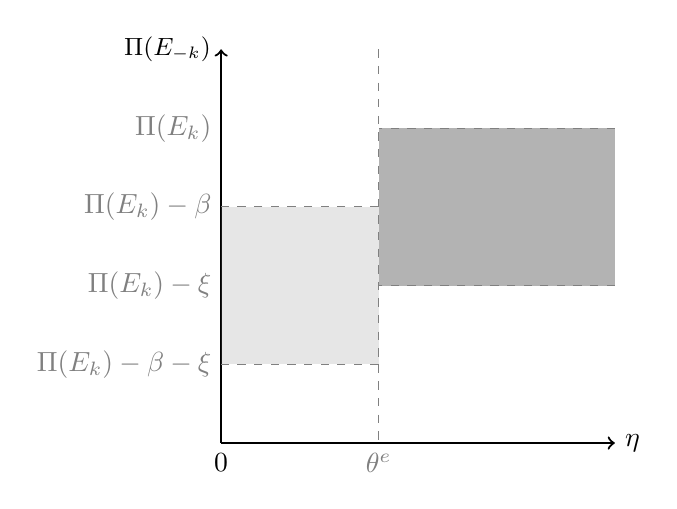
\begin{tikzpicture}
         \draw[black, thick][->] (0,0) -- (5,0) node[right] {$\eta$};
         \draw[black, thick][->] (0,0) node[below]{0} -- (0,5) node[left] {\small{$\Pi(E_{-k})$}};
         \draw[gray, dashed] (2,5) -- (2,0) node[below] {$\theta^e$};
         \draw[gray, dashed] (2,1) -- (0,1) node[left] {$\Pi(E_k)-\beta-\xi$};
         \draw[gray, dashed] (5,2) -- (2,2);
         \draw[gray, dashed] (2,3) -- (0,3) node[left] {$\Pi(E_k)-\beta$};
         \draw[gray, dashed] (5,4) -- (2,4) ;
         \draw[gray] (0,2) node[left] {$\Pi(E_k)-\xi$};
         \draw[gray] (0,4) node[left] {$\Pi(E_k)$};
         \draw[draw=gray, draw opacity=0, fill=gray, fill opacity=0.2] (2,1)--(0,1)--(0,3)--(2,3) -- cycle;
         \draw[draw=gray, draw opacity=0, fill=gray, fill opacity=0.6] (2,2)--(5,2)--(5,4)--(2,4) -- cycle;
    \end{tikzpicture}}
\end{minipage}
\begin{minipage}{0.49\textwidth}
\centering
Si $\beta > \xi$

\scriptsize{
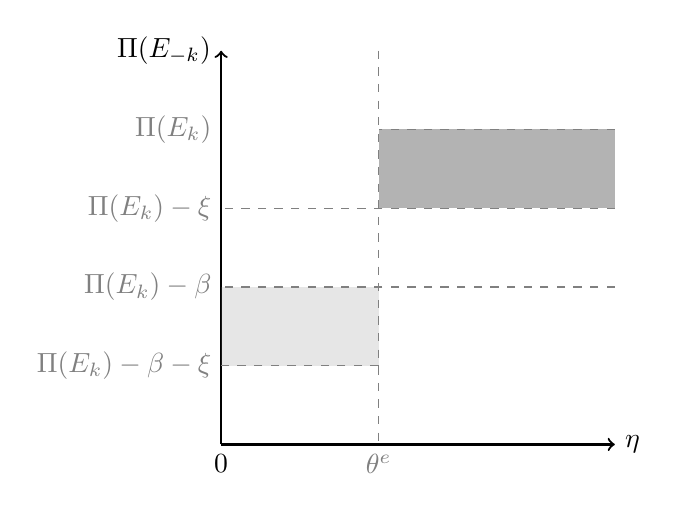
\begin{tikzpicture}
     \draw[black, thick][->] (0,0) -- (5,0) node[right] {${\eta}$};
     \draw[black, thick][->] (0,0) node[below]{0} -- (0,5) node[left] {$\Pi(E_{-k})$};
     \draw[gray, dashed] (2,5) -- (2,0) node[below] {$\theta^e$};
     \draw[gray, dashed] (2,1) -- (0,1) node[left] {$\Pi(E_k)-\beta-\xi$};
     \draw[gray, dashed] (5,2) -- (0,2) node[left] {$\Pi(E_k)-\beta$};
     \draw[gray, dashed] (5,3) -- (0,3) node[left] {$\Pi(E_k)-\xi$};
     \draw[gray, dashed] (5,4) -- (2,4) ;
     \draw[gray] (0,4) node[left] {$\Pi(E_k)$};
     \draw[draw=gray, draw opacity=0, fill=gray, fill opacity=0.2] (2,1)--(0,1)--(0,2)--(2,2) -- cycle;
     \draw[draw=gray, draw opacity=0, fill=gray, fill opacity=0.6] (2,3)--(5,3)--(5,4)--(2,4) -- cycle;
\end{tikzpicture}}
\end{minipage}
\label{fig:equilibrios}
\begin{minipage}{\textwidth}
    \centering
    \vspace*{0.5cm}
    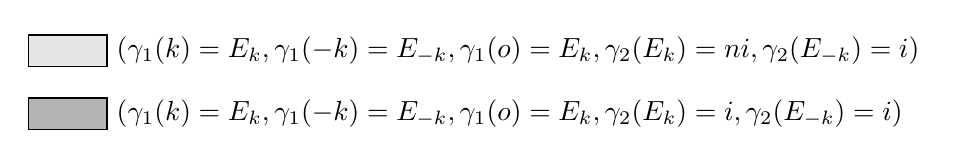
\begin{tikzpicture}
         \draw[draw=black, draw opacity=1, fill=gray, fill opacity=0.2] (1,0.8)--(0,0.8)--(0,1.2)--(1,1.2) -- cycle;
         \draw[black] (1,1) node[right] {$(\gamma_1(k)=E_k, \gamma_1(-k)=E_{-k}, \gamma_1(o)=E_k, \gamma_2(E_k)=ni, \gamma_2(E_{-k})=i)$};
         
         \draw[draw=black, draw opacity=1, fill=gray, fill opacity=0.6] (1,0)--(0,0)--(0,0.4)--(1,0.4) -- cycle;
         \draw[black] (1,0.2) node[right] {$(\gamma_1(k)=E_k, \gamma_1(-k)=E_{-k}, \gamma_1(o)=E_k, \gamma_2(E_k)=i, \gamma_2(E_{-k})=i)$};
         
    \end{tikzpicture}
\end{minipage}
\begin{singlespace}
    \floatfoot{\footnotesize{\textit{Nota:} La figura representa los equilibrios separadores del modelo. $E_k$ es la acción que toma el jugador 1 de identidad binaria $k$ y el jugador de identidad no binaria. $E_{-k}$ es la acción que toma el jugador 1 de identidad binaria $-k$. $\beta$ es el costo que percibe el jugador 1 de no interactuar con el jugador 2. $\xi$ es el costo de violar uno mismo la norma social. $\eta$ es el costo que percibe el jugador 2 de no interactuar con el jugador 1, y $\theta^e$ es el costo esperado por el jugador 2 de que el jugador 1 esté violando la norma social.}\par}
\end{singlespace}
\end{figure}
\vspace*{0.5cm}
\vfill
\begin{framed}
\noindent Sea $\gamma_j$ la estrategia del jugador $j$, y  sea $k \in \{F,M\}$,

\noindent (i) $(\gamma_1(k)=E_k, \gamma_1(-k)=E_{-k}, \gamma_1(o)=E_k, \gamma_2(E_k)=ni, \gamma_2(E_{-k})=i)$ es equilibrio si $\eta\in(0, \theta^e) \wedge \Pi_1(E_{k})- \beta \geq \Pi_1(E_{-k}) \geq  \Pi_1(E_{k})- \beta - \xi$

\noindent (ii) $(\gamma_1(k)=E_k, \gamma_1(-k)=E_{-k}, \gamma_1(o)=E_k, \gamma_2(E_k)=i, \gamma_2(E_{-k})=i)$ es equilibrio si $\eta\in[\theta^e, \infty) \wedge \Pi_1(E_{k}) \geq \Pi_1(E_{-k}) \geq \Pi_1(E_{k})- \xi$
\end{framed}

En resumen, la primera condición para que los jugadores lleguen a un equilibrio separador es que las personas de identidad binaria se adhieran a la norma social. Si esa condición se cumple, el equilibrio puede ser de dos tipos. El primer equilibrio sucede si el costo esperado de ver que se está violando la norma social es mayor al costo de no interactuar. En ese caso el jugador 2 solo interactúa con el jugador 1 si este le manda una señal que le de certeza de cuál es su identidad de género. El segundo equilibrio sucede si el costo de no interactuar es mayor al costo esperado de ver que se viola la norma social. En ese caso, el jugador 2 interactúa con el jugador 1 sin importar si cree que está violando la norma social. 

Si se da el primer o el segundo equilibrio depende de los parámetros poblacionales, los cuales puedes variar entre sociedades y tipo de interacción. Por ejemplo, se espera que el costo de ver que se viola la norma social sea mayor en sociedades más conservadoras, como el estado de Mississippi o entre los miembros del Opus Dei. Mientras que, se espera que ese mismo costo sea menor en sociedades más liberales, como el estado de California o el barrio Santa Fe, en Bogotá. También, el costo de no interactuar puede variar dependiendo de tipo de interacción o el propósito de la misma. Por ejemplo, no interactuar cuando la interacción puede llevar a formar una empresa, es más costoso a dejar de interactuar cuando la interacción sería estar cerca en el transporte público. 

Estas condiciones de los equilibrio son contrastadas con el experimento que presenta la siguiente sección. 
